% =============================================================================
% Lecture 11, Part 2: Bayesian Statistics II --- Hierarchical Models
% ECON 8310: Business Forecasting
% University of Nebraska at Omaha
% =============================================================================

\documentclass[aspectratio=169, 11pt]{beamer}

\input{header}

\title[Hierarchical Models]{Bayesian Statistics II --- Hierarchical Models}
\subtitle{ECON 8310: Business Forecasting --- Lecture 11, Part 2}
\author{Department of Economics}
\institute{University of Nebraska at Omaha}

% =============================================================================
\begin{document}
% =============================================================================

\begin{frame}
  \titlepage
\end{frame}

\begin{frame}{Lecture Outline}
  \tableofcontents
\end{frame}

% =============================================================================
\section{Which Series May Be Pooled}
% =============================================================================

\sectionslide{Which Series May Be Pooled}{%
  Before you pool anything, ask what the groups have in common.}

% --- Slide: the problem -----------------------------------------------------
\begin{frame}{The Question}
  \textbf{Does demand rise in weeks when SNAP benefits are disbursed, and by how much --- store by
  store?} Homework 3's memo assumed those differences were real. First, a check that needs no
  model: SNAP is a \emph{food} program.
  \begin{center}
    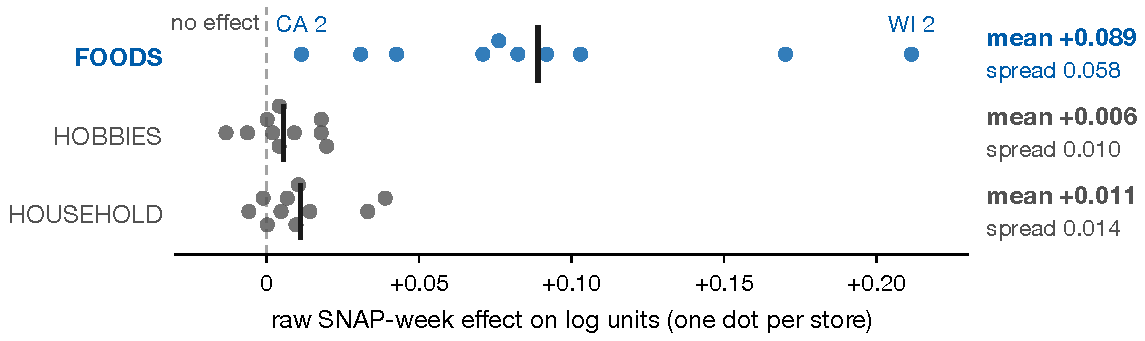
\includegraphics[height=3.75cm]{../Figures/Lecture11_Part2/question_strip.pdf}
  \end{center}
  \vspace{-0.3cm}
  \textbf{These are not thirty versions of the same thing.} FOODS responds; the other two barely
  move. Pooling all thirty would tell the model they are interchangeable.

  \vspace{0.05cm}
  \muted{\footnotesize\itshape Each dot: one series, high-SNAP weeks minus the rest, mean log
  units, 277 weeks. Spread: SD across stores.}
\end{frame}

% --- Slide: exchangeability -------------------------------------------------
\begin{frame}{Exchangeability: the Assumption Under Every Hierarchy}
  \begin{definitionbox}{Exchangeable}
    Groups are \textbf{exchangeable} when, before seeing the data, you have no reason to expect
    one to differ from another in a particular direction. Swapping their labels would not change
    what you believe.
  \end{definitionbox}

  \vspace{0.1cm}
  The ten FOODS stores qualify: nobody could say in advance which store's SNAP effect is largest.
  FOODS against HOBBIES does \textbf{not}: a food program moves food.

  \vspace{0.15cm}
  \textbf{Today:} the \textbf{ten FOODS series}, five thinned to \textbf{8 weeks}. That imbalance
  is the point.

  \vspace{0.1cm}
  \muted{\footnotesize\itshape The lab pools all thirty anyway, and measures what it costs.}
\end{frame}

% --- Slide: two bad options -------------------------------------------------
\begin{frame}{Complete Pooling and No Pooling}
  Within that exchangeable set there are two obvious approaches, and each fails in a different
  direction.
  \begin{center}
    {\small
    \begin{tabular}{p{3.0cm}p{4.4cm}p{4.9cm}}
      \toprule
      & \textbf{What it does} & \textbf{How it fails} \\
      \midrule
      \textbf{Complete pooling} & One SNAP effect for all ten series. \newline
      \texttt{b = pm.Normal("b", 0, 1)} & Denies that stores differ at all. A genuinely
      different store is averaged away. \\[3pt]
      \textbf{No pooling} & A separate effect per series, estimated independently. \newline
      \texttt{shape=10} & A series with 8 weeks gets an estimate built from 8 weeks. Mostly
      noise, reported as a finding. \\
      \bottomrule
    \end{tabular}
    }
  \end{center}

  \vspace{0.05cm}
  \textbf{You have used both already without naming them.} Homework 3's random forest pooled all
  thirty series into one model with store dummies --- close to complete pooling. Homework 1
  fitted ARIMA to one series at a time --- no pooling. The choice has always been made by
  convenience; partial pooling makes it a modeling decision and lets the data settle it.
\end{frame}

% =============================================================================
\section{Partial Pooling}
% =============================================================================

\sectionslide{Partial Pooling}{%
  Let each series have its own effect --- drawn from a shared distribution
  the data also estimates.}

% --- Slide: the hierarchy ---------------------------------------------------
\begin{frame}{The Hierarchy Is One Extra Line}
  Give each series its own effect $b_j$, but say where those effects come from:
  \[
    b_j \sim \mathcal{N}(\mu_b,\ \sigma_b), \qquad j = 1, \ldots, 10
  \]
  \vspace{-0.25cm}

  $\mu_b$ is the typical SNAP effect across FOODS, and $\sigma_b$ is \textbf{how much stores
  genuinely differ}. Crucially, both are estimated from the data rather than assumed.

  \begin{center}
    {\small
    \begin{tabular}{p{3.1cm}p{9.2cm}}
      \toprule
      $\sigma_b \rightarrow 0$ & The model concludes stores do not differ, and reproduces
      complete pooling. \\[3pt]
      $\sigma_b$ large & The model concludes they differ a lot, and approaches no pooling. \\[3pt]
      In between & Each $b_j$ is pulled toward $\mu_b$ --- \emph{how far} depending on how much
      data that series has. \\
      \bottomrule
    \end{tabular}
    }
  \end{center}

  \vspace{0.05cm}
  \textbf{That last row is the whole idea.} A series with 277 weeks barely moves; one with 8 weeks
  moves a long way. Nobody chose those weights --- they fall out of the model.
\end{frame}

% --- Slide: shrinkage intuition ---------------------------------------------
\begin{frame}{Why This Is the Right Answer, Not a Compromise}
  Partial pooling sounds like splitting the difference. It is better than that.

  \vspace{0.15cm}
  With 8 observations, a series' own estimate is mostly noise. Pulling it toward $\mu_b$ is the
  right response, not a fudge: you would not call a coin biased after three flips.

  \begin{keybox}
    \textbf{Regularization, for the sixth time.} The prior shrinks each group toward $\mu_b$ as
    Ridge shrinks coefficients toward zero --- but the strength, $\sigma_b$, is \emph{estimated},
    not tuned by cross-validation.
  \end{keybox}

  \vspace{0.1cm}
  \muted{\footnotesize\itshape Smoothing penalty (L3) $\rightarrow$ pruning (L4) $\rightarrow$
  \texttt{reg\_lambda} (L5) $\rightarrow$ Ridge and LASSO (L6) $\rightarrow$ weight decay (L7)
  $\rightarrow$ hierarchical priors.}
\end{frame}

% =============================================================================
\section{Fitting It, and the Trap}
% =============================================================================

\sectionslide{Fitting It, and the Trap}{%
  The obvious code does not work, and the reason
  is geometry rather than statistics.}

% --- Slide: PyMC ------------------------------------------------------------
\begin{frame}{The Model in PyMC}
  \begin{examplebox}{Non-centered hierarchical model}
    {\tiny\linespread{1.05}\selectfont
    \texttt{with pm.Model() as model:}\\
    \texttt{\mbox{}\ \ mu\_b = pm.Normal("mu\_b", 0, 0.5)\ \ \ \ \ \ \ \# typical SNAP effect}\\
    \texttt{\mbox{}\ \ sd\_b = pm.HalfNormal("sd\_b", 0.25)\ \ \ \ \ \# how much stores differ}\\
    \texttt{\mbox{}\ \ z\ \ \ \ = pm.Normal("z", 0, 1, shape=J)\ \ \ \ \# non-centered}\\
    \texttt{\mbox{}\ \ b\ \ \ \ = pm.Deterministic("b", mu\_b + z * sd\_b)}\\[2pt]
    \texttt{\mbox{}\ \ a = pm.Normal("a", y.mean(), 1, shape=J)\ \ \# per-series level}\\
    \texttt{\mbox{}\ \ s = pm.Exponential("s", 1.0)}\\[2pt]
    \texttt{\mbox{}\ \ pm.Normal("obs", mu=a[idx] + b[idx]*snap, sigma=s, observed=y)}
    }
  \end{examplebox}
  \texttt{J} is the number of series (10). \texttt{idx} maps each row to its series, so
  \texttt{b[idx]} picks out the right effect for every observation. That indexing pattern is how every hierarchical model in PyMC is written.

  \vspace{0.15cm}
  \textbf{Note what is \emph{not} here.} No decision about how much to pool, no weighting scheme,
  no threshold for ``enough data.'' Those all come out of estimating $\sigma_b$.
\end{frame}

% --- Slide: the funnel ------------------------------------------------------
\begin{frame}{The Trap: Write It the Obvious Way and It Breaks}
  The natural way to write the hierarchy is \texttt{b = pm.Normal("b", mu\_b, sd\_b, shape=J)}
  --- the \emph{centered} form, which reads exactly like the equation. On our data it produces:
  \begin{center}
    {\small
    \begin{tabular}{lrrl}
      \toprule
      & \textbf{Centered} & \textbf{Non-centered} & \textbf{Want} \\
      \midrule
      Divergences & \textbf{43} & \textbf{0} & 0 \\
      $\hat{R}$ & 1.003 & 1.003 & $< 1.01$ \\
      ESS (bulk) & 966 & 1{,}719 & $> 400$ \\
      \bottomrule
    \end{tabular}
    }
  \end{center}

  \vspace{0.05cm}
  \textbf{Only one alarm fires.} $\hat{R}$ and ESS pass; on those alone you would ship it.
  \textbf{43 divergences against a threshold of zero} is the objection to trust.

  \vspace{0.15cm}
  \muted{\footnotesize\itshape Counts move with the seed, and even with the machine. Ten more seeds:
  15--285 divergences centered, 0--11 non-centered; $\hat{R}$ or ESS objected in 2 of the 11 runs,
  divergences in all 11.}
\end{frame}

% --- Slide: the funnel, and the change of coordinates -------------------------
\begin{frame}{Why It Breaks: a Funnel}
  Every posterior draw for one thin series (CA\_1), against $\sigma_b$ on a log axis:
  \begin{center}
    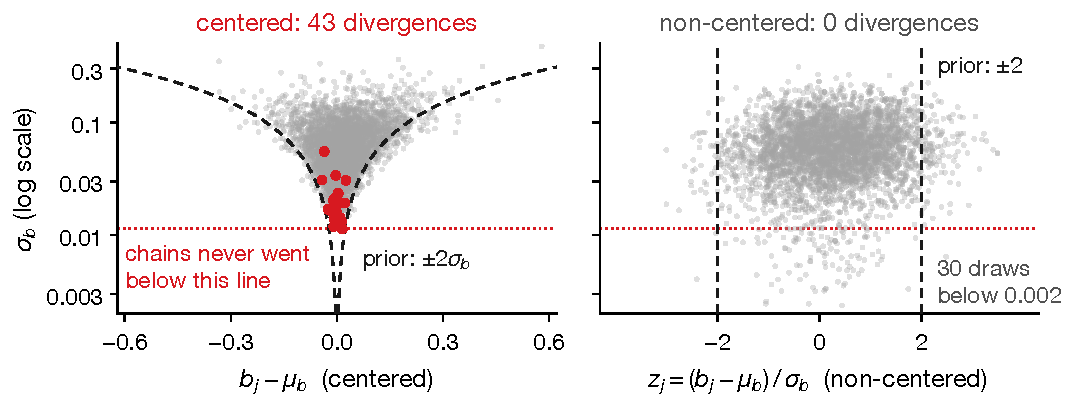
\includegraphics[height=4.1cm]{../Figures/Lecture11_Part2/funnel.pdf}
  \end{center}
  \vspace{-0.3cm}
  {\small Given $\sigma_b$, the prior spreads $b_j - \mu_b$ by $\sigma_b$: a funnel, pinched where
  $\sigma_b$ is small. The divergences sit in the neck (39 of 43 in the bottom tenth of $\sigma_b$),
  and the chains go no lower. $b_j = \mu_b + \sigma_b z_j$ is a change of coordinates: $z_j$ spreads
  by 1 at every height, a column the sampler can walk. Exact for the prior; the posterior follows
  closely.}

  \vspace{0.05cm}
  \muted{\footnotesize\itshape Posterior geometry matters \parencite[§4.6.1]{MartinKumarLao2021}.}
\end{frame}

% =============================================================================
\section{Reading the Result}
% =============================================================================

\sectionslide{Reading the Result}{%
  Shrinkage, measured --- and checked against
  data the model never saw.}

% --- Slide: the measurement -------------------------------------------------
\begin{frame}{Shrinkage, Measured}
  Each series' own (unpooled) estimate, and where the hierarchy moved it:
  \begin{center}
    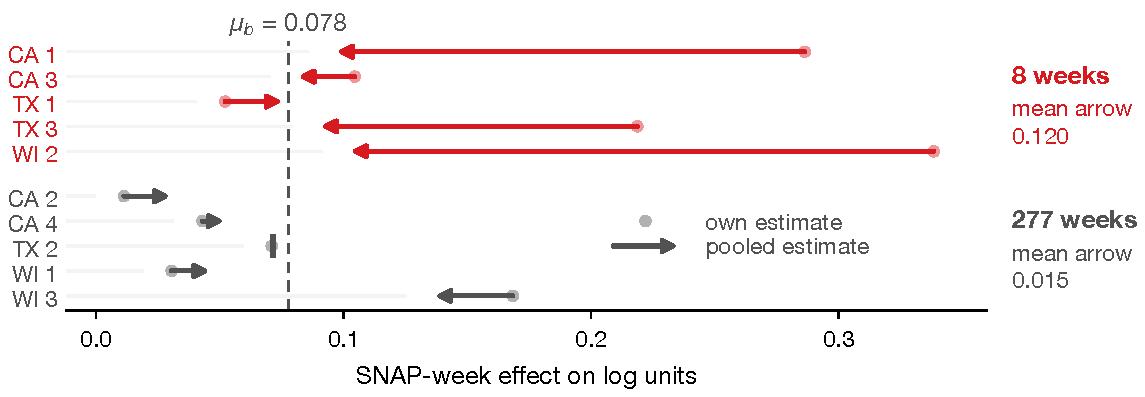
\includegraphics[height=4.1cm]{../Figures/Lecture11_Part2/shrinkage_arrows.pdf}
  \end{center}
  \vspace{-0.3cm}
  \textbf{Thin series moved 8.1 times further toward $\mu_b$}, though nobody said which were thin.
  Full series keep most of their spread ($0.055 \rightarrow 0.037$); thin ones lose it
  ($0.108 \rightarrow 0.010$).

  \vspace{0.05cm}
  \muted{\footnotesize\itshape Each pooled estimate sits approximately at a precision-weighted
  point between $\mu_b$ and its own: thin series keep about a tenth of theirs, full series about
  three-quarters. Only approximately, because $\mu_b$ and $\sigma_b$ are integrated over.}
\end{frame}

% --- Slide: held-out check --------------------------------------------------
\begin{frame}{Checked Against Data the Model Never Saw}
  The weeks we thinned from CA\_1, CA\_3, TX\_1, TX\_3 and WI\_2 still exist. Each ring is the
  SNAP effect observed in them:
  \begin{center}
    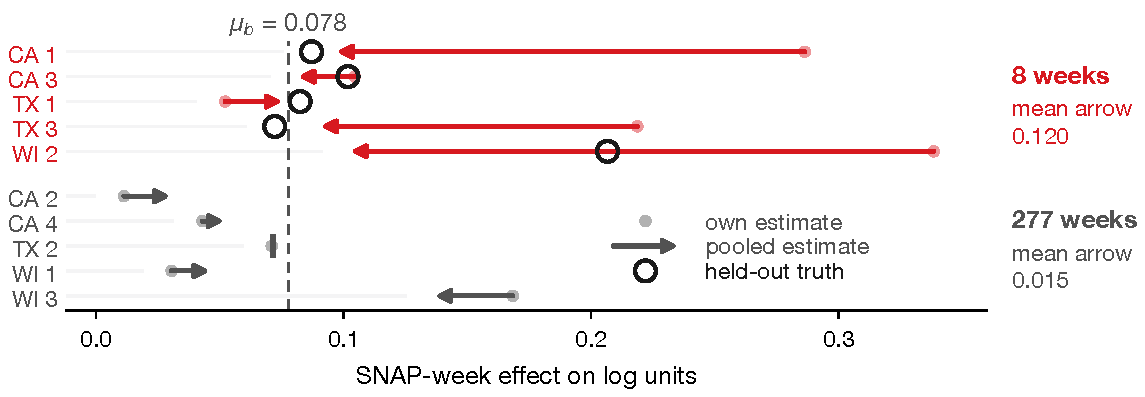
\includegraphics[height=4.1cm]{../Figures/Lecture11_Part2/shrinkage_heldout.pdf}
  \end{center}
  \vspace{-0.3cm}
  \textbf{RMSE against the truth: 0.126 unpooled, 0.048 pooled --- 2.6 times smaller.} Pooling won
  on four series of five; CA\_3 lost narrowly. WI\_2 was pulled past its truth, yet still ended
  closer than its own estimate.

  \vspace{0.05cm}
  \muted{\footnotesize\itshape Borrowing strength is not a figure of speech: the thin series were
  estimated better \emph{because} the other five existed.}
\end{frame}

% --- Slide: the business answer ---------------------------------------------
\begin{frame}{What the Model Actually Concluded}
  The estimated hierarchy: $\mu_b = 0.078$ (94\% HDI about $[0.02,\ 0.15]$) and
  $\sigma_b = 0.065$.

  \vspace{0.1cm}
  So a SNAP week lifts FOODS units by about \textbf{8\%}, and stores genuinely differ around that
  by about \textbf{7 percentage points}.

  \begin{warningbox}
    \textbf{Not a license for store-by-store stocking.} The thin stores' own estimates ran from
    $5\%$ to $40\%$. The held-out weeks say that was mostly noise; $\sigma_b = 0.065$ says not
    \emph{all} of it.
  \end{warningbox}

  \vspace{0.1cm}
  \textbf{The defensible plan:} 8\% everywhere, modest store variation around it, and no store's
  own estimate until it has the weeks to support one.
\end{frame}

% =============================================================================
\section{Key Takeaways}
% =============================================================================

\sectionslide{Key Takeaways}{%
  What hierarchy buys, and what it costs.}

\begin{frame}{Lecture 11, Part 2: Key Takeaways}
  \begin{keybox}
    {\footnotesize
    \begin{enumerate}\itemsep2pt
      \item \textbf{Ask what may be pooled first:} groups must be \textbf{exchangeable}. FOODS
            and HOBBIES are not.

      \item \textbf{Complete pooling} denies groups differ; \textbf{no pooling} reports noise as a
            finding.

      \item \textbf{Partial pooling} draws each group's parameter from a shared distribution
            whose spread is estimated.

      \item \textbf{Shrinkage is proportionate:} thin series moved \textbf{8.1$\times$} further;
            held-out error was \textbf{2.6$\times$} smaller.

      \item \textbf{Regularization for the sixth time}, with the strength estimated, not tuned.

      \item \textbf{Write it non-centered.} 43 divergences became 0: same model, a change of
            coordinates.
    \end{enumerate}
    }
  \end{keybox}
  \muted{\itshape Next: Bayesian linear regression --- coefficients as distributions.}
\end{frame}

\begin{frame}[allowframebreaks]{References}
  \printbibliography[heading=none]
\end{frame}

\end{document}
